\subsection{Project Timeline}
\subsubsection*{Gantt Chart}
\todomessage{Gantt Chart}

\todomessage{Cumulative hours}

\subsubsection*{Task Revisions and Additions}
\todomessage{Modifications to Gantt from Scope}

\begin{itemize}
	\item Revisions to the original scope of works [BLANK] have been highlighted in orange.
	
	\item Discuss revisions....

\end{itemize}

\subsection{Major Problems and Issues}
\begin{itemize}
	\item Vibrations and stability: In semester 1, more time than initially planned was spent on eliminating vibrations and increasing stability of the aircraft. 
	
	\item Printer repair: Many hours have been spent fixing and tweaking the 3D printer.  During the holidays, a week of testing and repair was done to fix an issue with clogged nozzles. See gant chart xxx
	
	\item Multiple crashes: Crashes throughout the year required the purchase of replacements parts, and corresponding delays due to shipping time. Large amounts of time were then spent re-testing components. All major crashes were due to faulty hardware such as the power module, RC transceiver and failure of a motor, resulting in the fixed-wing flight controller not being fully tested. See Gantt chart and flight tests xxx.
	
	\item Team Member Departure: Shanon was unable to make meaningful contributions after semester 1, including mid year break, particularly during the final weeks before the submission of final report. Several sections of the Gantt chart remain incomplete as a result of this.
\end{itemize}
\todomessage{Reference Gantt}

\subsection{Project Diary}
The team has made extensive use of Trello to maintain records of the tasks performed throughout the project. The project's records/diary may be viewed in full detail here: \url{https://trello.com/uavoutbackchallenge2016}.

\subsection{`Flight Tests}
\label{sec:diary}
 The Gantt chart cannot fully express the amount of ongoing testing (including flight tests) and iterative design that was performed every week of each semester. Therefore the table below in no way captures all flight tests that were performed, but only major flights outside of university and tests leading up to them. 
\begin{table}[!htbp]
	\centering
	\caption{Flight tests performed by \ID}
	\begin{tabular}{|c|c|c|c|c|c|c|}
		\hline Date & Location & Flight Time & Aim & Result & Problems \\ 
		\hline 13/05/15 & Melb Uni & 2 min & Courtyard Winged Hover test & Complete & - \\ 
		\hline 02/07/15 & Melb Uni & 2 min & Courtyard Alt-Hold test & Complete & - \\ 
		\hline 03/07/15 & Cardinia & 15 min & Major test/Autotune & Complete & Radio cut outs \\ 
		\hline 27/07/15 & Cardinia  & 0 min & Autotune new firmware & Incomplete & Radio faillure \\ 
		\hline 31/07/15 & Cardinia  & 6 min & Autotune new firmware & Crash & Motor burnt out, damage  \\ 
		\hline 22/08/15 & Cardinia  & 2 min & Autotune new firmware & Crash & Power Module Failure, damage\\
		\hline 04/09/15 & Melb Uni & 1 min & Courtyard Alt-Hold test & Complete & - \\  
		\hline 05/09/15 & Cardinia  & 8 min & Autotune new firmware & Complete & Back gear broken\\
		\hline 18/07/15 & Melb Uni & 1 min & Courtyard Alt-Hold test & Complete & - \\  
		\hline 19/09/15 & Cardinia  & 10 min & Test flight with wings & Complete & Overheating \\ 
		\hline 27/09/15 & Cardinia  & 5 min & Test transition & Incomplete & Solder melting (overheating) \\ 
		\hline 
	\end{tabular} 
	\label{tab:tests}
\end{table}

\subsection{Scope of Works}
\label{sec:scope}
See below for the final version of team \ID Scope of Works.
\includepdf[pages=2-]{scope.pdf}